\chapter{Background and Related Work}
\label{ch:background}

This section provides basic information on the main terminology used for this work. This will include technical concepts and a brief description for each term, and define what we understand in relation to this current work. Understanding Large Language Models (LLMs) and how it evolved to angentic llm with its different architectures to leverage them in real-world applications is paramount to understand our approach and solution proposal for developing and smart autonomously operating LEGO train.
Because the system is intended to operate entirely on a Raspberry Pi 4, with no external cloud access, the technologies used need to be efficient, compact, and designed for resource-limited hardware. The most important components include smaller versions of large language models (LLMs) suitable for tool calling, local message passing systems such as ZeroMQ, and agentic architectures that support decision making.

%
% Section: Der erste Abschnitt - Background 
%

\section{Background} % Terminologyerklaeung 
\label{sec:background:first_section}

\subsection{Large Language Models (LLM)}
\label{subsec:background:first_section:first_subsection}

Large language models (LLMs) are deep neural network architectures designed to understand and generate natural human language. They excel in tasks such as recognizing, summarizing, translating, predicting, and generating text. Typically, they have been pre-trained on vast amounts of text data and fine-tuned for specific usage. They rely on transformer architectures, which allow them to analyze relationships across tokens in a flexible way \cite{vaswani_attention_2023, brown_efficient_2023}. Their ability to complete sentences and generate text makes them perfect for applications where human-computer interaction through conversational bot can be achieved. Thanks to significant GPT-4's advances in understanding context, nuance, and complex queries \cite{mapletoft_attempt_2024, cao_automatic_2024}, usage of natural language processing applications has been skyrocketing (e.g. Deepl, Google Assistant and customor service chatbots). Their widespread application in various fields indicates their transformative potential in technology, education, healthcare, and more \cite{wang_survey_2024}.

However, "LLMs do not possess genuine understanding or reasoning akin to human cognition" \cite{li_survey_2024}. Because they operate by just predicting the next word in a sequence based on patterns from their training data (statistical reasoning), they have a high tendency to potentially "hallucinate" or give false or misleading information. Additionally, it is known that these models tend to be biased, which raises concerns by many.

It cannot be denied, that most state-of-the-art LLMs require considerable memory and compute, often running into the tens of gigabytes. Several strategies help reduce this overhead. One is \textbf{quantization}, where the model weights are stored in low precision (e.g., 4-bit or 8-bit), which makes inference faster and less memory-intensive (\cite{dettmers2022optimizers}). Another approach is known as \textbf{knowledge distillation}, in which a smaller model learns from a bigger one by mimicking its outputs (\cite{hinton2015distilling}). \textbf{Pruning} is also commonly used: it involves removing connections in the neural network that do not contribute much to performance (Han et al., 2016). When used together, these methods allow for the deployment of LLMs on edge devices such as Raspberry Pi with acceptable speed and accuracy \cite{zhang-kennedy_systematic_2021}

\subsection{Retrieval-Augmented Generation (RAG) Architectures}
\label{subsec:background:first_section:second_subsection}

Retrieval-Augmented Generation (RAG) is an architectural paradigm that combines LLMs with retrieval systems, enabling the model to access external information sources while generating responses. This approach significantly enhances the model's accuracy and relevance, especially in scenarios requiring up-to-date or domain-specific information. For example, LLMs can utilize a RAG system to pull relevant data from databases or documents during query processing, thus improving the quality of generated text for user inquiries \cite{wang_survey_2024, jeong_adaptive-rag_2024}.


\begin{description}
    \item[RAG Architecture] The fundamental RAG architecture involves retrieving relevant documents from a knowledge base (indexed and ingesting data from a source, usually happening offline) and combining that retrieved information with the generative capabilities of LLMs to produce contextually enriched responses.

    \item[Conditional RAG (CRAG)] This variant incorporates conditional features that refine the retrieval process by focusing on user-specific conditions or prompts (tailored user intent). This increases the effectiveness of the interaction by ensuring that the responses provided are more personalized and context-aware.

    \item[Self-RAG] Self-RAG involves models that can autonomously identify when external information is needed and retrieve it as part of their operational flow. This type of architecture further enhances the reasoning capability of the model, allowing it to assess its current task and decide when additional context or data is warranted for optimal performance (Rong et al., 2024; Yang et al., 2024).
\end{description}


\subsection{Agentic LLMs} 
\label{subsec:background:first_section:third_subsection}

While regular LLMs and RAGs can generate responses, agentic LLMs can go further. Think of them as a natural language processing unit with autonomous decision-making capabilities. They reason, call tools they need to achieve their goal, and are able to perform actions in a sequence. In addition, they learn from the environment or previous outcomes (\cite{yao_react_2023}; \cite{xi_rise_2023}). These models behave more like autonomous software agents. The "agentic" term suggests an integrated architecture in which LLMs not only generate text but also action taking and the use of external tools based on user queries and interact with their environment effectively (\cite{li_advanced_2024}, \cite{li_review_2024}). This capability clears the the for development of systems that can participate in collaborative environments, making them suitable for applications such as digital assistants and automation in software development.

There are many ways to structure such systems. The ReAct (Reason and Act) framework, for example, combines internal reasoning and external tool usage in a loop. LangGraph takes a modular approach: It treats workflows as graphs, where each node can represent a tool, a memory update, or a decision point (\cite{langchain_agent_2024}). Other architectures like AutoAgent (\cite{tang_autoagent_2025}) offer full no-code agent environments, though they tend to be too large for embedded use. SmolAgents (\cite{kumari_smolagents_2025}) is much smaller and easier to deploy, but has limited planning ability. Frameworks such as ModelScope-Agent and AgentScope emphasize multi-agent communication and tool chaining, but often require stronger infrastructure.

In summary, agentic LLMs represent pivotal advances in the field of artificial intelligence, particularly in natural language processing \cite{matthew_berman_ai_2024, ibm_technology_ai_2024, don_woodlock_using_2025}. With their enhanced capabilities, they promote a new wave of intelligent agents capable of reasoning, adapting, and interacting effectively with users. The ongoing research and development in this domain holds considerable promise in creating more sophisticated AI applications capable of transforming user experiences across various sectors. For this current project, a balance between simplicity, customizability, and performance is required. LangGraph fits well in this middle ground due to its modular Python design and clear agent workflow logic. See section \autoref{subsec:background:first_section:first_subsection} 

\begin{figure}[H]
    \centering
    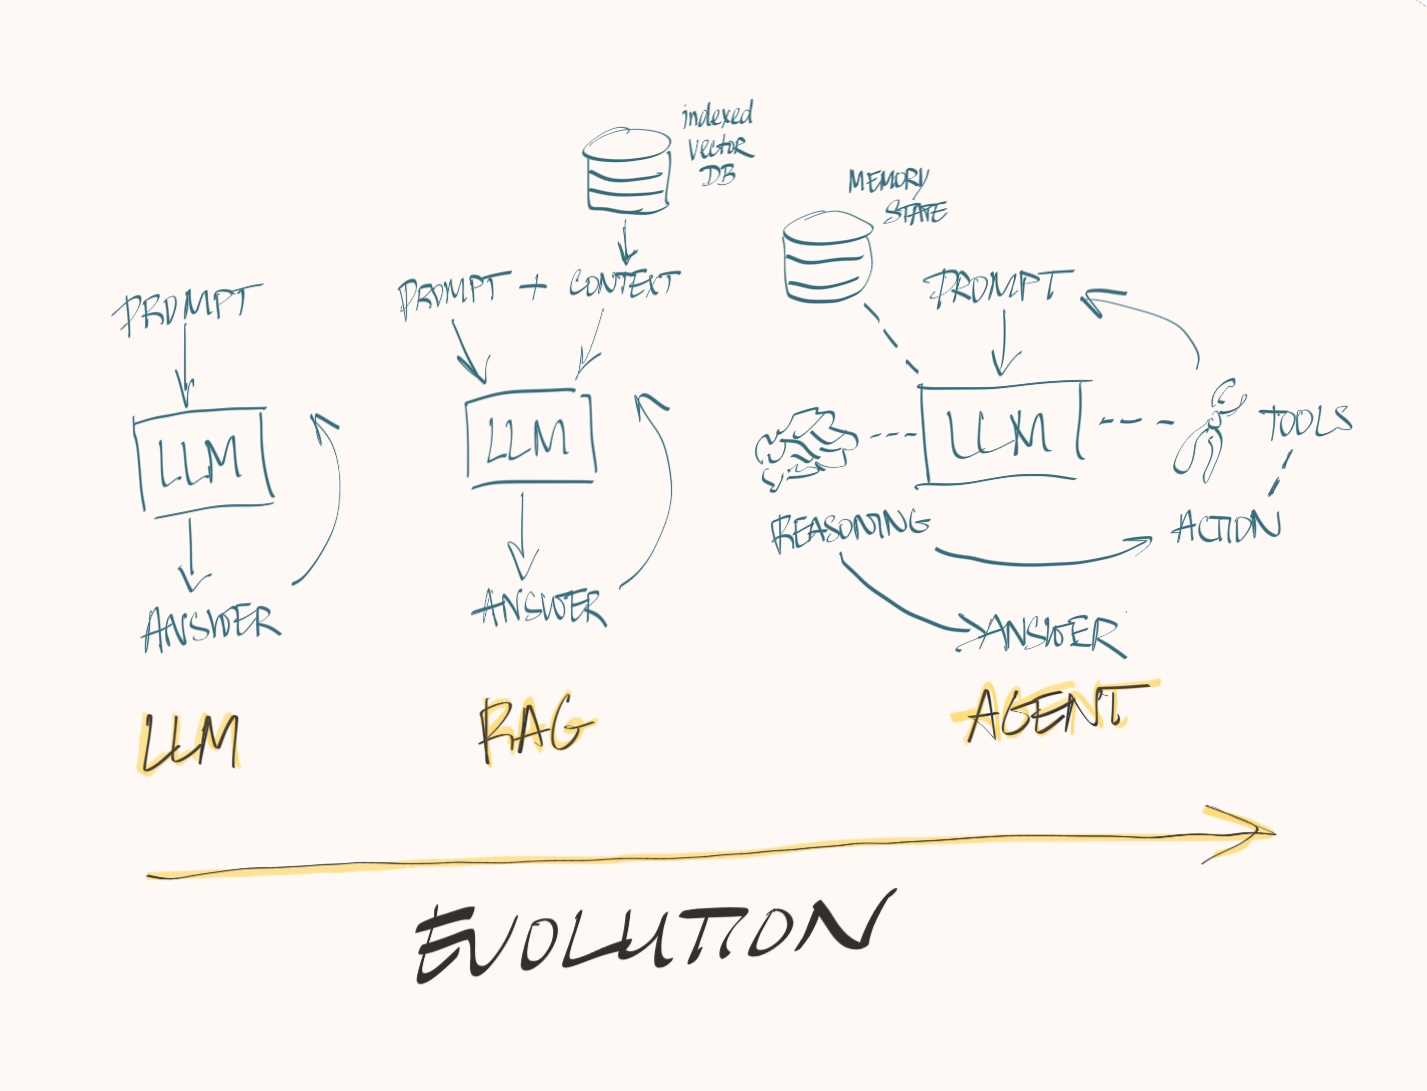
\includegraphics[width=\textwidth]{docs/llm_evolution.jpg}
    \caption{Evolution of LLM}
\end{figure}



\subsection{ZeroMQ for Local Communication}
\label{subsec:background:first_section:third_subsection}

Running several processes in parallel, namely a vision system, a voice recognizer, and a command execution of a LEGO train motor — requires communication. However, using Internet-based protocols like HTTP introduces latency and dependency. ZeroMQ is a lightweight messaging library that supports asynchronous communication between local processes without a central broker \cite{hintjens_zeromq_2013}. It supports flexible messaging patterns such as pub-sub and push-pull, which are ideal for small-scale distributed systems. ZeroMQ is frequently used in robotics and IoT applications for exactly this reason: it provides low-latency messaging and decouples components, increasing system robustness and fault tolerance \cite{wang_survey_2024, zhang-kennedy_systematic_2021}.


%
% Section: Der Zweite Abschnitt
%

\section{Related Work}
\label{sec:background:second_section} 

In this section we will give an overview of related works. For this we conducted an preliminary intensive literature research with the help of elicit, to be found in the appendix. We consulted it and derived most relevant sources. We will discuss this in detail in \ref{sec:background:second_section:first_subsection} 

Many research efforts have tackled similar challenges, such as running intelligent agents on edge devices, enabling offline control systems, and integrating LLMs with hardware. This section presents both academic work and open source frameworks reviewed to make a inform to realise the goal of this project.

% -------------------------------------------------
\subsection{Overview of Agentic Frameworks}
\label{subsec:background:first_section:first_subsection}

\begin{description} 
\item[\cite{yao_react_2023}]
This paper presents \textbf{ReAct}, a method for combining reasoning and actions inside LLMs. Instead of just generating answers, the model thinks through steps and takes actions in between. This structure makes it more reliable and interpretable. It worked really well in tasks like answering complex questions or navigating websites. I found this idea very useful as it shows how agentic behavior can be achieved without needing lots of training or hardware.

\item[\cite{asai_self-rag_2023}]
In this work, the authors introduce \textbf{Self-RAG}, which builds on retrieval-augmented generation by adding self-reflection. Basically, the model reflects on what it retrieved and decides if the info is useful before answering. This was tested on various question-answering and fact-checking tasks, and it outperformed other methods. This idea is interesting for edge cases, where every response needs to be more accurate because of limited retries.

\item[\cite{xi_rise_2023}]
This survey gives a very broad \textbf{overview of LLM-based agents,} from their design to how they can work together in groups. It even talks about things like social behavior in agent societies. I liked that it broke agents down into brain, perception, and action components. It helped me understand where my train control system fits into this bigger picture. They also discuss challenges with evaluation and generalization, which was helpful when deciding on a framework.

\item[\cite{jeong_adaptive-rag_2024}]
Jeong et al. suggest using a classifier to predict how hard a question is, and then select the right retrieval strategy. So the system doesn't waste resources on easy queries, and still handles harder ones properly. I think this is a smart way to optimize performance, especially when running locally. It avoids the “one size fits all” approach and adapts based on what’s needed.

\item[\cite{yan_corrective_2024}]
This paper focuses on improving what happens when document retrieval fails. The authors propose \textbf{CRAG}, a setup where the model can judge the quality of the retrieved data, and take action to fix it, like re-querying or using broader search. It also filters irrelevant info from the retrieved documents. This seems really helpful for systems that work offline or have limited memory, where the first retrieval might be bad.

\item[\cite{li_review_2024}]
Li's paper gives an \textbf{overview of three common agent techniques}: using tools, planning steps, and learning from feedback. What I found most useful was the idea of breaking systems into reusable modules (called LMPCs). It made me think more carefully about building the AI agent as components that can be reused later, like the voice input or the logic for stopping the train.

\item[\cite{paramanayakam_less_2024}]
The authors suggest that giving too many tools to a language model is inefficient. So, they propose a \textbf{smart tool selection method} that only shows the model a few tools at a time. This saves energy and time — they saw big improvements in speed and power use. I thought this paper supported the idea that it's okay to limit features if you can make smarter choices.

\item[\cite{dong_generalizing_2024}]
This paper combines an \textbf{LLM with a driving model} by letting the LLM make occasional high-level decisions, while a simpler model drives the car. It's like splitting the brain and the reflexes. This saves compute and works better in real-time. Even though this was about cars, I saw a lot of overlap with how I structured the train controller, where the LLM just decides what to do, but doesn’t touch the motor directly.

\item[\cite{huang_efficient_2024}]
Here, the authors built a system where \textbf{multiple units with LLMs} explain what’s happening on the road, in real time. Each unit uses environment and movement data to describe and reason about events. It was cool to see how they used prompt engineering to get better behavior without changing the model. This gave me ideas on how to handle narration or error feedback in my own project.

\item[\cite{tang_autoagent_2025}]
\textbf{AutoAgent} is a very advanced system that lets you build agents using just natural language. It comes with its own file manager, tool engine, and logic planner. The downside is that it's really resource-hungry. While it was impressive, I realized quickly it wouldn't fit on a Raspberry Pi. Still, I used it as a reference for what kinds of features matter when designing smaller agents.

\item[\cite{kumari_smolagents_2025}]
Kumari \textbf{compares LangGraph and SmolAgents}. SmolAgents is super lightweight and good for Pi-like setups but doesn’t support memory or planning. LangGraph supports branching and memory, but is a bit heavier. I agree with the conclusion: LangGraph is better if you want structure and flexibility, especially for projects like mine where logic and reactions matter.
\end{description}

%\begin{landscape}
    \begin{table}[htbp]
    \centering
    \caption{Comparison of Selected Agentic LLM Frameworks for Edge Deployment}
    \label{tab:framework_comparison}
    \resizebox{\textwidth}{!}{%
    \begin{tabular}{|l|l|c|c|c|l|l|l|}
        \hline
        \textbf{Framework} & \textbf{Architecture Type} & \textbf{Tool Use} & \textbf{Open Source} & \textbf{Edge-Ready} & \textbf{Workflow Support} & \textbf{Optimization} & \textbf{Limitations} \\
        \hline
        LangGraph & Graph-based workflows & Yes & Yes & Partial & Conditional branching, persistent memory & Modular Python design & Not pre-optimized for Pi; requires tuning \\
       
        SmolAgents & Minimalist agent & Yes & Yes & Yes & Linear (no memory/planning) & Extremely low resource usage & Lacks advanced decision-making and context retention \\
        
        AutoAgent & Zero-code agent OS & Yes & Yes & No & Full planning and memory & Rich features, but heavy runtime & Too resource-intensive for Raspberry Pi \\
        
        TinyAgent & Quantized tool caller & Yes & Partial & Partial (e.g., tested on higher-end devices) & None (only basic function calls) & 4-bit quantization for speed & No structured workflow or memory support \\
        
        Promp-tAI & LLM deployment infrastructure & No & Yes & Yes & None & Docker-based, optimized for inference & Does not offer agent logic or planning \\
        \hline
    \end{tabular}%
    }
    \end{table}
%\end{landscape}


% -------------------------------------------------
\subsection{Five Promising Frameworks}
\label{subsec:background:second_section:second_subsection}

\subsubsection{Top Frameworks in Detail}

\paragraph{LangGraph.} This framework allows agents to be defined as a graph of actions, memory updates, or tool calls. It supports branching logic and tool orchestration while maintaining a small enough footprint to potentially run on a Pi, especially when paired with quantized LLMs \cite{langchain_agent_2024, kumari_smolagents_2025}.

\paragraph{SmolAgents.} Designed for extremely low-resource environments, SmolAgents use minimal logic and quick tool calls. However, they lack long-term memory and planning capabilities, limiting their usefulness for complex tasks \cite{kumari_smolagents_2025, xi_rise_2023}.

\paragraph{AutoAgent.} A powerful, no-code environment for developing and deploying multi-agent workflows. It includes memory, file systems, and planning logic, but is too resource-heavy for embedded devices \cite{tang_autoagent_2025}.

\paragraph{TinyAgent.} A lightweight function-calling agent using 4-bit quantized models. Though efficient and responsive, it does not support memory, and limited public information makes integration difficult \cite{erdogan2024tinyagent}.

\paragraph{Promp-tAI.} A tool designed to deploy LLMs on edge devices using containerization. While helpful for infrastructure, it lacks agentic features like decision-making or tool use \cite{nezami2024promptai}.


% -------------------------------------------------
\subsubsection{ASR and Vision for Embedded AI}

Offline ASR on the Pi can be achieved using Vosk, which supports real-time speech-to-text without internet access \cite{vosk2023api}. For visual perception, lightweight models like YOLOv5 Nano and TensorFlow Lite enable object detection with 5–10 FPS on the Raspberry Pi \cite{lin2022realtime, tan2023lightweightcv}.


% -------------------------------------------------
\subsubsection{Educational Robotics and Constructivism}

This project continues previous student work at Hochschule Darmstadt using LEGO and Raspberry Pi platforms. While earlier versions relied on simple color sensors and MQTT-based control, this study introduces AI-based autonomy. The pedagogical foundation follows Papert's constructivist theory \cite{papert1980mindstorms}, where learning occurs through creation and experimentation. Related literature supports robotics as a powerful tool for fostering creativity and digital fluency in educational contexts \cite{resnick2009kindergarten,bers2020coding}.

% -------------------------------------------------
\subsection{Identified Gaps and Framework Justification}

Many frameworks either lack flexibility or are too demanding for embedded systems. SmolAgents is easy to deploy but too basic. AutoAgent supports complex agents but requires more memory than the Pi can provide. TinyAgent is fast but lacks planning. Promp-tAI assists with deployment but has no logic layer.

LangGraph stands out for its support of memory, conditional logic, and modular tools. It is also written in Python and designed to be extensible. When used with lightweight LLMs, LangGraph provides a practical foundation for building a responsive, voice- and vision-enabled train control agent on a Raspberry Pi.

% -------------------------------------------------
\section{Research Questions and Study Significance}
\label{sec:background:third_subsection:researchquestions}

After reviewing existing work on embedded AI systems and agentic LLM architectures, this study is guided by the following research questions, each rooted in the constraints and requirements of our real-world LEGO train system.
\begin{description}
    \item[RQ1:] \textit{How can agentic LLMs be deployed on resource-limited devices like the Raspberry Pi while still providing reliable performance for real-time control tasks?}\\
    
    Running an LLM on a Raspberry Pi locally presents clear challenges: low RAM, no GPU, and limited CPU power. This question investigates whether techniques such as quantization \cite{dettmers2022optimizers}, pruning \cite{han2016deep}, or the use of smaller open-source models (e.g., LLaMA variants) can support agentic behavior locally. In our setup, we use a quantized Ollama llama3-groq-tool-use model that can handle voice commands and make control decisions without cloud assistance. The agent must respond immediately, e.g., to stop the train if an obstacle appears on the track. Therefore, the inference time must be less than 1 to 3 seconds to be useful. The question is not just "can it run?" but "can it run fast enough to be useful?"
    
    \item[RQ2:] \textit{What communication architecture supports real-time coordination between an AI agent, object detection, and train motor control on a single edge device?} \\
    
    Instead of relying on frameworks like ROS or MQTT, this project uses ZeroMQ for its lightweight, brokerless decentralized design \cite{hintjens2013zeromq,zhang2021zeromqiot}. Components like the ASR module, the object detection process, and the train motor controller run in separately and communicate asynchronously using pub-sub patterns. This avoids blocking issues and allows the system participants to remain responsive even if one module slows down. The communication layer plays a critical role in making sure that decisions are made and executed reliably and in order, especially when reacting to safety-critical events.

    \item[RQ3:] \textit{How can simple but effective safety logic be implemented in a low-resource, autonomous control system?} \\
    
    Rather than complex reinforcement learning or advanced anomaly detection, our system focuses on lightweight, rule-based safety mechanisms. For example, the object detection module triggers a stop signal if an object is within a predefined proximity threshold. The LLM agent also considers recent context (via LangGraph memory) to prevent repeated or unsafe actions. Although there are more advanced safety techniques, this question looks at what can be achieved with limited compute and basic vision tools such as YOLOv5 Nano or TensorFlow Lite \cite{lin2022realtime,tan2023lightweightcv}.
\end{description}


%-------------------------------
\subsubsection{Study Significance}
\label{sec:background:third_subsection:study_significance}

To best of our knowledge this project offers a practical example of how to build a local, private, and low-cost intelligent control system; something that is still underexplored in real-world educational or prototyping contexts. The main value lies in how accessible and flexible the system is.

\begin{itemize}
  \item \textbf{Replicable:} It uses common hardware (Raspberry Pi, LEGO, USB mic), and all software is open-source.
  \item \textbf{Modular:} Components are separate and can be improved or replaced without rewriting the entire system.
  \item \textbf{Privacy-respecting:} No internet or cloud services are not required, which is valuable for school projects or sensitive environments.
  \item \textbf{Educational:} Students can explore Python coding, agent logic, voice control, asynchronous networking and safety protocols in one system.
  \item \textbf{Constructivist:} Based on hands-on experimentation and modular tinkering, the system aligns well with project-based learning approaches \cite{papert1980mindstorms,resnick2009kindergarten}.
\end{itemize}

By combining LLM reasoning, real-time inputs, and local tool control, the prototype creates opportunities for both exploration and practical deployment in constrained settings.

